\documentclass[border=5pt]{standalone}
\usepackage{pgfplots}
\usepgfplotslibrary{groupplots}
\pgfplotsset{compat=1.18}

\definecolor{blue}{HTML}{2166AC}
\definecolor{orange}{HTML}{D6604D}
\definecolor{green}{HTML}{1B7837}
\definecolor{gold}{HTML}{C99400}
\definecolor{rose}{HTML}{B2182B}
\definecolor{gray}{HTML}{6C757D}

\begin{document}
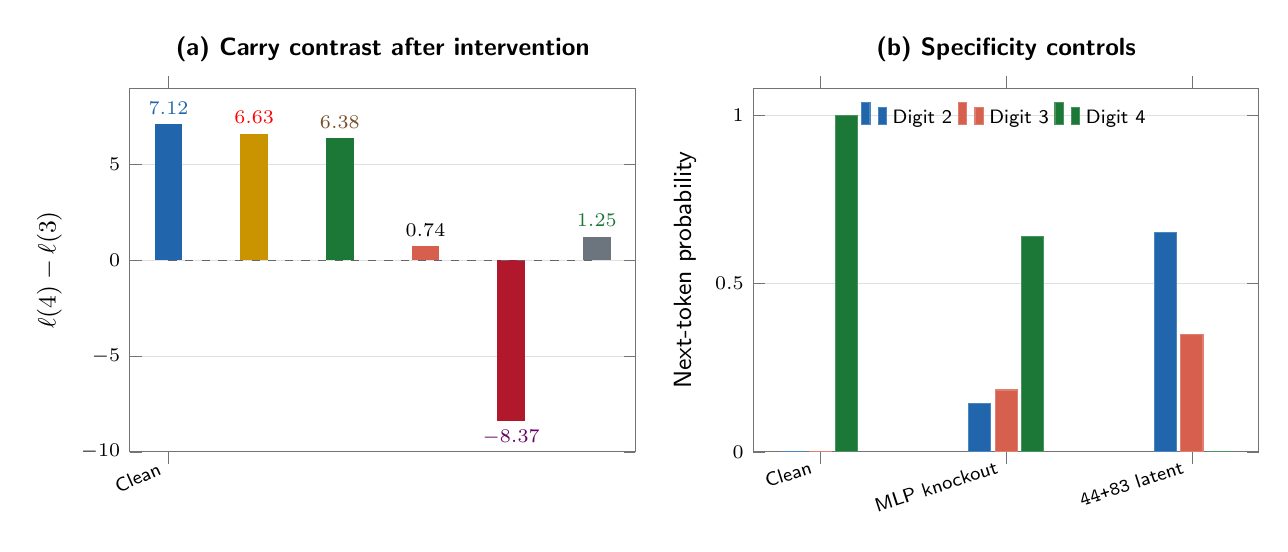
\begin{tikzpicture}
\begin{groupplot}[
    group style={group size=2 by 1, horizontal sep=1.5cm},
    width=8.0cm,
    height=6.2cm,
    ymajorgrids,
    grid style={draw=black!12},
    axis line style={draw=black!55},
    tick label style={font=\sffamily\scriptsize},
    label style={font=\sffamily\small},
    title style={font=\sffamily\small\bfseries},
    legend style={font=\sffamily\scriptsize, draw=none, fill=none},
]

\nextgroupplot[
    title={(a) Carry contrast after intervention},
    ybar,
    bar width=10pt,
    ymin=-10,
    ymax=9,
    ylabel={$\ell(4)-\ell(3)$},
    symbolic x coords={Clean,Sparse,Full1,Full2,Raw,Knockout},
    xtick=data,
    xticklabels={Clean,Sparse 73,Full $\alpha=1$,Full $\alpha=2$,Raw MLP,MLP knockout},
    x tick label style={rotate=24,anchor=east},
    enlarge x limits=0.09,
    nodes near coords,
    nodes near coords style={font=\sffamily\scriptsize},
]
\addplot+[draw=none, fill=blue, bar shift=0pt] coordinates {(Clean,7.12)};
\addplot+[draw=none, fill=gold, bar shift=0pt] coordinates {(Sparse,6.63)};
\addplot+[draw=none, fill=green, bar shift=0pt] coordinates {(Full1,6.38)};
\addplot+[draw=none, fill=orange, bar shift=0pt] coordinates {(Full2,0.74)};
\addplot+[draw=none, fill=rose, bar shift=0pt] coordinates {(Raw,-8.37)};
\addplot+[draw=none, fill=gray, bar shift=0pt] coordinates {(Knockout,1.25)};
\draw[black!60, dashed] (axis cs:Clean,0) -- (axis cs:Knockout,0);

\nextgroupplot[
    title={(b) Specificity controls},
    ybar=1.5pt,
    bar width=8pt,
    ymin=0,
    ymax=1.08,
    ylabel={Next-token probability},
    symbolic x coords={Clean,Knockout,AltSource},
    xtick=data,
    xticklabels={Clean,MLP knockout,\texttt{44+83} latent},
    x tick label style={rotate=18,anchor=east},
    enlarge x limits=0.18,
    legend columns=3,
    legend style={at={(0.5,0.98)},anchor=north},
]
\addplot+[fill=blue, draw=blue!80] coordinates {
    (Clean,0.0003) (Knockout,0.1426) (AltSource,0.6523)
};
\addlegendentry{Digit 2}
\addplot+[fill=orange, draw=orange!80] coordinates {
    (Clean,0.0008) (Knockout,0.1836) (AltSource,0.3477)
};
\addlegendentry{Digit 3}
\addplot+[fill=green, draw=green!80] coordinates {
    (Clean,1.0000) (Knockout,0.6406) (AltSource,0.0001)
};
\addlegendentry{Digit 4}

\end{groupplot}
\end{tikzpicture}
\end{document}
